\chapter{Implementation}
\label{cha:implementation}

For the implementation of our algorithm, we use the distributed framework Apache Spark\footnote{http://spark.apache.org/}. In this chapter, we will firstly introduce some knowledge about spark and how we use these techniques to implement our model. After that, we will introduce the experiments we did and analysis our results.


\section{Introduction of Spark}


Spark was developed by \cite{ZahariaChowdhuryEtAl2010} and has many useful features for the parallel execution of programs. As the basic datastructure it has the 
\gls{RDD} % RDD
(Resilient Distributed Dataset). The RDD is a special data structure containing the items of a dataset, e.g. sentences or documents. Spark automatically distributes these items over a cluster of compute nodes and manages its physical storage. 

Spark has one driver and several executors. Usually, an executor is a cpu core, and we call each machine as worker, so each worker has several executors. But logically we only need the driver and the executors, only for something about tuning we should care about the worker stuff, e.g. some operations need to do communication between different machines. But for most of cases, each executor just fetches part of data and deals with it, and then the driver collects data from all executors.

The Spark operations can be called from different programming languages, e.g. Python, Scala, Java, and R. For this thesis we use Scala to control the execution of Spark and to define its operations.

Firstly, Spark reads text file from file system (e.g. from the unix file system or from HDFS, the Hadoop file system) and creates an RDD. An RDD usually is located in the RAM storage of the different executors, but it may also stored on (persisted to) disks of the executors. Spark operations follow the functional programming approach. There are two types of operations on RDDs: \emph{Transformation operations} and \emph{action operations}.  A transformation operation transforms  a RDD to another RDD. Examples of transformation operations are map (apply a function to all RDD elements), filter (select a subset of RDD elements by some criterion), or sort (sort the RDD items by some key). Note that an RDD is not mutable, i.e. cannot be changed. If its element are changed a new RDD is created. 

Generally after some transformation operations, people use action operations to gain some useful information from the RDD. Examples of action operations are count (count the number of items), reduce (apply a single summation-like function), aggregate (apply several summation-like functions), and collect (convert an RDD to a local array). 
 


\section{Implementation}

We use $syn0$ to represent the input embedding $V$ and $syn1$ to represent the output embedding $U$. $syn0$ and $syn1$ are defined as broadcast variables, which are only readable and can not be changed by executors. When they are changed in a training step copies are returned as a new RDD. 

\paragraph{Gradient Checking}\

Firstly we set a very small dataset mutually and calculate empirical derivative computed by the finite difference approaximation derivatives and the derivative computed as our model shows from last chapter. The result shows the difference between these two derivative is very small. So our gradient calculation is correct.

\paragraph{Data preparing} \

We use the same corpus as other papers used, a snapshot of Wikipedia at April, 2010 created by \cite{Shaoul2010}, which has 990 million tokens. Firstly we count the all words in the corpus. We transform all words to lower capital and then generate our vocabulary (dictionary). And then we calculate the frequency of word count. For example, there are 300 words which appear 10 times in the corpus. So the frequency of count 10 is 300. From this we can calculate the accumulated frequency. That is, if the accumulated frequency of count 200 is 100000, there would be 100000 words whose count is at least 200. This accumulated frequency can be used to select a vocabulary $D$ with the desired number of entries, which all appear more frequent than $minCount$ times in the corpus.  If the count of a word is smaller than $minCount$ we remove it from corpus, so it won't be in the vocabulary.  The following 4 figures (Figure \ref{fig:1to51},Figure \ref{fig:51to637},Figure \ref{fig:637to31140} and Figure \ref{fig:31140torest}) show the relationship between accumulated frequency and word count. To make visualization more clear, we display it as four different figures with different ranges of word count. And with some experience from other papers (\citep{HuangSocherEtAl2012}, \citep{TianDaiEtAl2014} and \citep{NeelakantanShankarEtAl2015}), in some of our experiments we set $minCount=20$ and others have $minCount=200$. Actually, when word count is 20, the accumulated frequency is 458142, that is the vocabulary size would be 458142; when word count is 200, the accumulated frequency is 95434, that is the vocabulary size would be 95434.


\begin{figure}[H]
\centering
    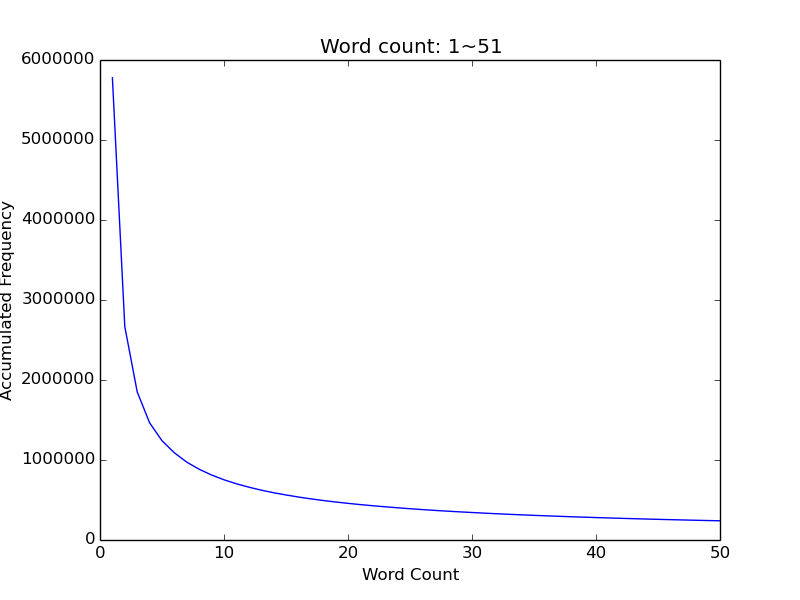
\includegraphics[width=0.75\textwidth]{1to51} 
	\caption{Shows the accumulated frequency of word count in range [1,51]}
	\label{fig:1to51}
\begin{figure}[H]
\centering
  \end{figure}
        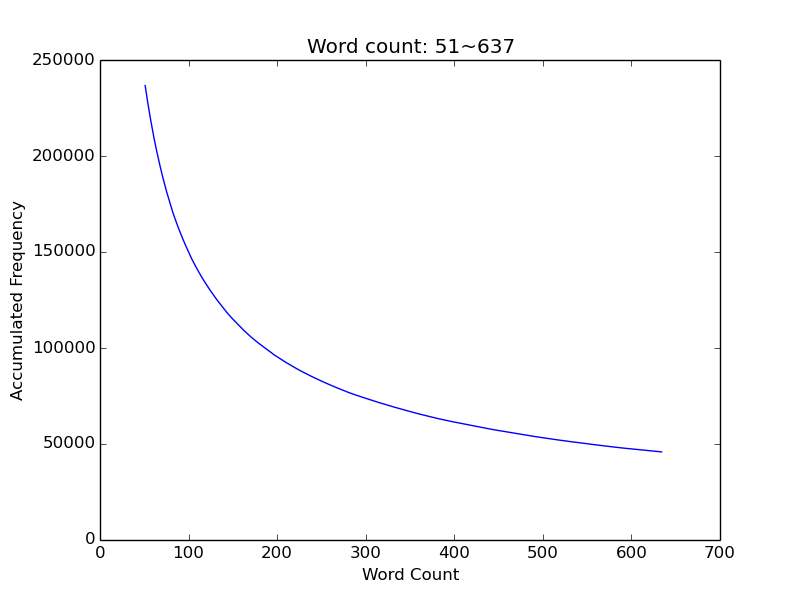
\includegraphics[width=0.75\textwidth]{51to637} 
	\caption{Shows the accumulated frequency of word count in range [51,637]}
	\label{fig:51to637}
\end{figure}


\begin{figure}[H]
\centering
 	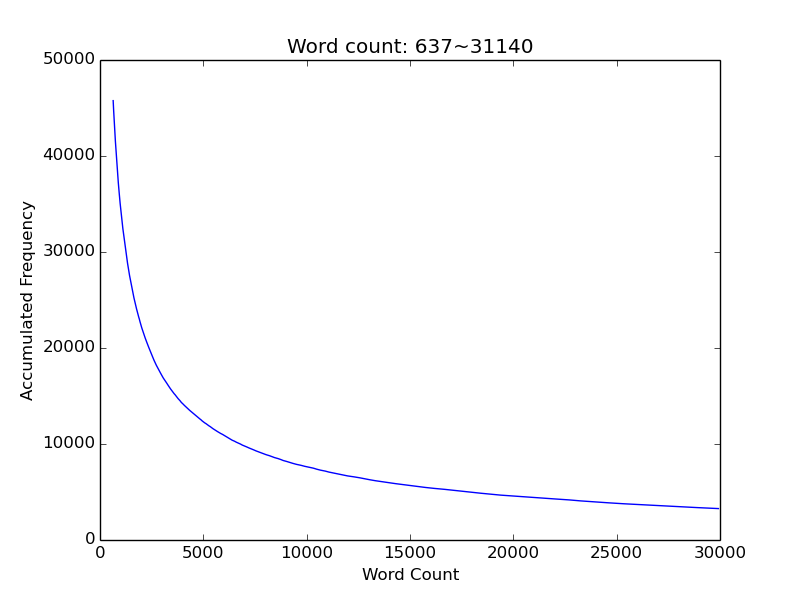
\includegraphics[width=0.75\textwidth]{637to31140} 
	\caption{Shows the accumulated frequency of word count in range [637,31140]}
	\label{fig:637to31140}
\begin{figure}[H]	
\end{figure}
\centering
	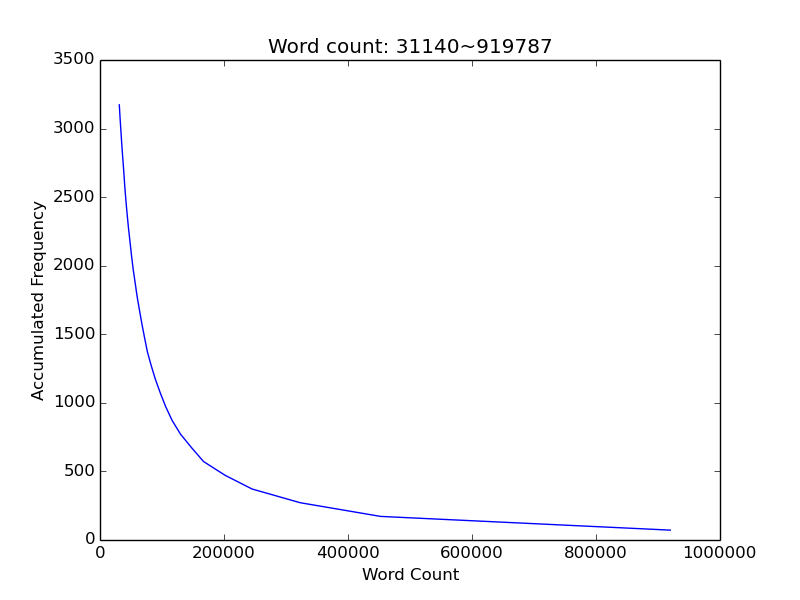
\includegraphics[width=0.75\textwidth]{31140torest} 
	\caption{Shows the accumulated frequency of word count in range [637,919787]}
	\label{fig:31140torest}
\end{figure}

\paragraph{Computing Environment} \ 

Our program is running on a single machine with 32 cores. For some experiments, we use all cores as executers. We also tried some experiments on a compute cluster of several machines, but the time of collecting parameters ($syn0$ and$syn1$) is too slow and actually too many executors actually is not really good for our program. After learning parameters parallel by stochastic gradient, the program collects all parameters and calculates the average, which reduces the learning effect and slow down the convergence especial when the number of executors is too many, although more executors can speed up training more or less.

\paragraph{Training set and validation set} \ 

We split the corpus into a training set and a validation set. The training set has $99\%$ of the data and validation set has only $1\%$ of the data. We use the validation set to monitor our training process if it is converging. If the training algorithm  converges, the loss of validation set should be at the lowest value. And then it gradually increases, which means the training is over-fitting. So we calculate the loss of the validation set after several training iterations and then compare with the previous validation loss. If the current value is bigger than previous value, we stop our training process and fetch the previous result as the final result to store to the disk. That is, after each calculation of the loss of validation set, we store our results. 

Note that, the validation set and training set should not be overlapping, because we use the validation set to monitor our training. And another import thing is that, the negative samples of validation set should always be fixed to reduce variance.  The assignment step for the word senses of the validation set is almost the same as the one for training set. The only different thing is that the negative samples for each word of each sentence in the validation set are not changed. But for each iteration of sense assignment for sentences in the training set, the negative sampling are new. 


Another thing is that, for each iteration, we do not use the whole training set to assign senses and learn parameters. Instead we split the training set into several parts and each time we only fetch one data part to do sense assignment (Assign Step)and parameters learning (Learn Step). Specifically, the training set was split into $numRDD$ different RDDs, which were persisted to disk to allow execution of the training in RAM. $numRDD$ is the number of RDD to split training dataset.

\paragraph{Learning Rate Reduction}\

At the beginning of experiment, the learning rate is set to $lr$. After each iteration, the learning rate will be reduced with a reduction factor $gm$. Specifically, using $\alpha$ to represent current learning rate and $\alpha^\prime$ to represent the new learning rate, we have
$$\alpha^\prime=\alpha*gm$$

\paragraph{Iteration}\ 

As described before, the while training process include several iterations. At the beginning the program fetches the first RDD and then for next each iteration, the it fetches one of other RDDs orderly. After several iterations, the program finishes processing all RDDs, and for the next iteration (if not stopping) it will fetches the first RDD again and repeat the above . Each iteration contains the sense assignment, adjusting the sense probabilities for each word based on the assigned senses, learning parameters , collecting parameters using $treeAggregate$ and normalizing sense embeddings, and every operations are on training set. And in some iteration (not every), the program assigns senses on the validation set and stores the RDD data. In experiments we compare the time of each operation in an iteration, and find that comparing the time of learning parameters and the time of parameters collection, the time of other operations can be ignored. Define $t1$ as the average time of learning parameters in an iteration, $t2$ as the collecting parameters in an iteration, $t3$ as the average time of all operations in an iteration, $t4$ as the total training time and $iter$ as the total number of iterations. And we will do some analysis on these time in next chapter.

\paragraph{Assign Step}\ \\
In the assignment, we use map transformation to transform each sentence with senses information to another sentence with changed senses information. The sense with the lowes loss is selected. So one RDD is transformed to another RDD. In this process, $syn0$ and $syn1$ are constant and will be used (only read) to calculate the loss. 


\paragraph{Learn Step}\ \\
In the training, we also use a map transformation. Instead of transforming sentences to sentences, we transform the original sentence RDD into the two-element collection of the updated $syn0$ and updated $syn1$. We broadcast these variables to the local $syn0$ and $syn1$ in each executor, so that each executor has its own  copy of $syn0$ and $syn1$ and can update them independently. So each executor has copies of $syn0$ and $syn1$. And then we use $treeAggregate$ to collect all such vectors together from different executors (cpu cores).  In the aggregation operation, different $syn0$'s vectors add up together, and different $syn0$'s vectors add up together. Finally, by dividing by the the number of partitions, we get one global $syn0$ and one global $syn1$ in the driver. For now, we set them as new $syn0$ and $syn1$, which will be broadcasted again in the next iteration. 

\paragraph{Normalization}\ \\
After getting the new global $syn0$ and $syn1$, some values of some embeddings may be very big. Thus, we need to do normalization to avoid to big values. Our normalization method is very simple, which is to check all embeddings from $syn0$ and $syn1$ if their Euclidean length is bigger than 4. If that is the case we just normalize them to the new embeddings with length of 4.

